\usection{Lecture 14: Dynamic games with Incomplete information}
\newsection
\subsection*{Logistics}
\begin{enumerate}
    \item Project topic due Sunday.
\end{enumerate}
\subsection*{Recap}
\begin{enumerate}
    \item Dynamic games with complete information - subgame perfect NE
    \item Static games with incomplete information - Bayesian NE
\end{enumerate}

We shall introduce a concept of a Perfect Bayesian Equilibrium (PBE) for dynamic games with incomplete information, which intuitively is a combination of SPNE and BNE.
\begin{aexample}{}{}
        \begin{center}
            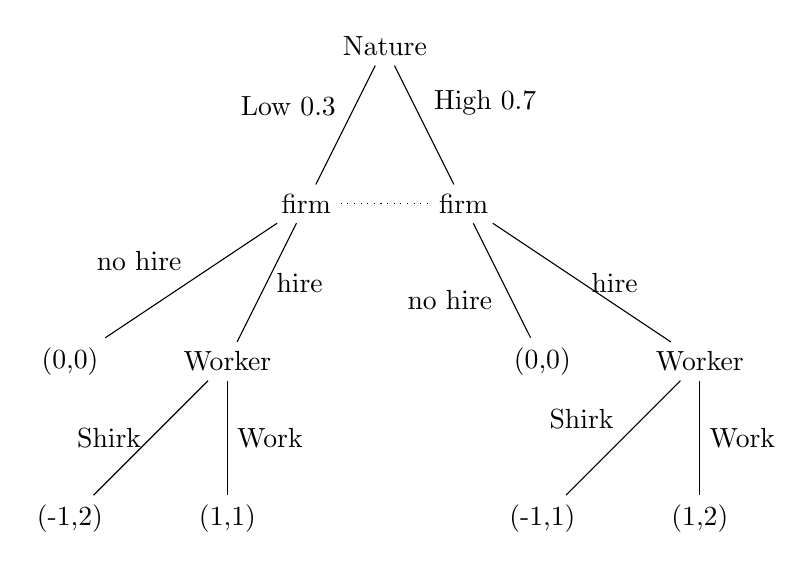
\begin{tikzpicture}
                \node (A) at (0,0){Nature};
                \node(B) at (-1,-2) {firm};
                \node(C) at (1,-2) {firm};
                \draw (A) edge  node[midway, above left]{Low 0.3}(B);
                \draw (A) edge  node[midway, above right]{High 0.7}(C);
                \draw[dotted] (B)--(C);
                
                \node(BB) at (-4,-4) {(0,0)};
                \node(CC) at (-2,-4) {Worker};
                \draw (B) edge  node[midway, above left]{no hire}(BB);
                \draw (B) edge  node[midway,  right]{hire}(CC);

                
                \node(BBB) at (2,-4) {(0,0)};
                \node(CCC) at (4,-4) {Worker};
                \draw (C) edge  node[midway,  below left]{no hire}(BBB);
                \draw (C) edge  node[midway,  right]{hire}(CCC);
                

                
                \node(DD) at (-4,-6) {(-1,2)};
                \node(EE) at (-2,-6) {(1,1)};
                \draw (CC) edge  node[midway, left]{Shirk}(DD);
                \draw (CC) edge  node[midway,  right]{Work}(EE);


                \node(DDD) at (2,-6) {(-1,1)};
                \node(EEE) at (4,-6) {(1,2)};
                \draw (CCC) edge  node[midway, above left]{Shirk}(DDD);
                \draw (CCC) edge  node[midway,  right]{Work}(EEE);
            \end{tikzpicture}
        \end{center}
\end{aexample}
Under this, there is a BNE where the worker always Shirks and the firm never hires. However, this is not an SPNE. A PBE would be that the high efficiency worker works if hired and a low one doesn't. Under this assumption, the payoff for hiring is\[
 0.3 (-1) + 0.7 (1) = 0.420>0
\]
so the firm hires.

\begin{aexample}{}{}
    \begin{center}
        \begin{tikzpicture}
            \node (A) at (0,0){1};
            \node(B) at (-1,-2) {2};
            \node(C) at (1,-2) {2};
            \node(special) at (3,0){(1,3)};
            \draw (A) edge node[midway, above]{R} (special);
            \draw (A) edge  node[midway, above left]{L}(B);
            \draw (A) edge  node[midway, above right]{M}(C);
            \draw[dotted] (B)--(C);
            
            \node(BB) at (-4,-4) {(2,1)};
            \node(CC) at (-2,-4) {(0,0)};
            \draw (B) edge  node[midway, above left]{L'}(BB);
            \draw (B) edge  node[midway,  right]{R'}(CC);

            
            \node(BBB) at (2,-4) {(0,2)};
            \node(CCC) at (4,-4) {(0,1)};
            \draw (C) edge  node[midway,  below left]{L'}(BBB);
            \draw (C) edge  node[midway,  right]{R'}(CCC);
            
        \end{tikzpicture}
    \end{center}
\end{aexample}
There are two NE: (L,L') and (R,R'). However the (R,R'), while a SPNE for the subgame starting at 1, does not make sense.
To capture this idea, we introduce this definition.

\definition{Continuation game}{
    A \textbf{continuation game} is a `subgame' that can start at any information set.

}
Furthermore, we attach ``beliefs'' for each node in an information set, and assume that players maximize their expected payoffs given beliefs.
Returning to the previous example, in the continuation game for $2$, the payoff for playing $L'$ for any belief is higher than $R'$, so is preferred in every scenario. Thus we can rule out the equilibrium (R,R').


In general, arbitrary beliefs do not work, for instance in the following example.

\begin{aexample}{}{}
    \begin{center}
        \begin{tikzpicture}
            \node (A) at (0,0){1};
            \node(B) at (-1,-2) {2};
            \node(C) at (1,-2) {2};
            \node(special) at (3,0){(1,3)};
            \draw (A) edge node[midway, above]{R} (special);
            \draw (A) edge  node[midway, above left]{L}(B);
            \draw (A) edge  node[midway, above right]{M}(C);
            \draw[dotted] (B)--(C);
            
            \node(BB) at (-4,-4) {(2,2)};
            \node(CC) at (-2,-4) {(2,1)};
            \draw (B) edge  node[midway, above left]{L'}(BB);
            \draw (B) edge  node[midway,  right]{R'}(CC);

            
            \node(BBB) at (2,-4) {(0,2)};
            \node(CCC) at (4,-4) {(0,5)};
            \draw (C) edge  node[midway,  below left]{L'}(BBB);
            \draw (C) edge  node[midway,  right]{R'}(CCC);
            
        \end{tikzpicture}
    \end{center}
\end{aexample}
Suppose that 2 puts a belief of $1$ that 1 chooses M, so will pick $R'$. But then 1, knowing 2's strategy, picks $L$. Then 2's best response is $L'$.

We need the beliefs to be consistent with the equilibrium play.

\definition{Perfect Bayesian Equilibrium}{
    A \textbf{Perfect Bayesian Equilibrium}
    consists of a set of action profiles (that possibly depend on history and type) and a belief system which specifies beliefs for every information set, such that \begin{itemize}
        \item The actions maximize the expected payoffs in every continuation game given the beliefs.
        \item The beliefs are consistent with the actions on `equilibrium path'.
    \end{itemize}
}
\begin{remark}
    In general, the consistency requirement means that the beliefs are given by Bayes' rule given the history and type.
\end{remark}
\begin{remark}
    The definition only talks about beliefs on the equilibrium path. Off path beliefs are arbitrary.
\end{remark}
\begin{aexample}{Signaling Game}{}
    Nature selects a type $t_i\in T$, and signals it to the sender. The sender sends a message $m_j\in M$ to the receiver. The receiver chooses an action $a_k\in A$. The payoffs are \[
        \pi_s(t_i,m_j,a_k), \pi_m(t_i,m_j,a_k)
    \]
    respectively.

    Some examples of signaling game model are \begin{enumerate}
        \item Job market signalling, where the type is the proficiency of the worker, the message is the CV, and the receiver is HR who decides to throws your application into the trash because it's a ghost job, yielding $\pi_s=\pi_m=0$ for everyone.
        \item Corporate investment, where the sender is a company that needs capital, the receiver is an investor. The signal is the likelihood of doing well, and the message is the guarantee of equity.
    \end{enumerate}

    \begin{center}
        \begin{tikzpicture}
            \node[label={right:N}] (start) at (0,0){\textbullet};
            \node[label={above:$t_1$}] (good) at (0,3){\textbullet};
            \node[label={below:$t_2$}] (bad) at (0,-3){\textbullet};
            \path (start) edgenode[midway,right]{0.5}(good);
            \path(start) edge node[midway,right]{0.5}(bad);

            \node (inv1) at (-3,3) {\textbullet};
            \node (inv2) at (-3,-3) {\textbullet};
            \node (inv3) at (3,3) {\textbullet};
            \node (inv4) at (3,-3) {\textbullet};

            \path[dotted] (inv1)edge node[midway, right]{receiver} (inv2);
            \path[dotted] (inv3)edge node[midway, right]{receiver} (inv4);
            

            \path (inv1) edge node[midway,above]{L} (good);
            \path (inv2) edgenode[midway,above]{L} (bad);
            \path (inv3) edge node[midway,above]{R}(good);
            \path (inv4) edge node[midway,above]{R}(bad);
            \node (one) at(-5,4){(1,3)};
            \node (two) at(-5,2){(4,0)};
            \node (three) at(-5,-2){(2,4)};
            \node (four) at(-5,-4){(0,1)};
            \node (five) at(5,4){(2,1)};
            \node (six) at(5,2){(0,0)};
            \node (seven) at(5,-2){(1,0)};
            \node (eight) at(5,-4){(1,2)};
            \path (inv1) edge   node [midway, above] {U} (one);
            \path (inv1) edge   node [midway, below] {D} (two);
            \path (inv2) edge   node [midway, above] {U} (three);
            \path (inv2) edge   node [midway, below] {D} (four);
            \path (inv3) edge   node [midway, above] {U} (five);
            \path (inv3) edge   node [midway, below] {D} (six);
            \path (inv4) edge   node [midway, above] {U} (seven);
            \path (inv4) edge   node [midway, below] {D} (eight);

        \end{tikzpicture}
    \end{center}
\end{aexample}
The sender can have a few strategies, always L, always R, L when $t_1$/ R when $t_2$, R when $t_1$/ L when $t_2$. The first two are known as pooling strategies while the last two are known as separating strategies.

We now go through the grueling process of looking at each strategy.
Suppose the message is always $L$, then the receiver chooses $U$ for better payoff. Now if the sender deviates and sends $R$, we need the receiver to have a belief system that results in playing $D$, so the payoff for deviating is negative. Solving this gives that the belief system for $(t_1,t_2) = (q,1-q)$ such that $q\leq 2/3$.


There is no pooling PBE for $R$.


Now if the sender sends $R$ for $t_1$ and $L$ for $t_2$, the receiver will choose $U$ in both cases using this belief that $(t_1,R)$, $(t_2,L)$ happen with probability 1. There is also no intiative for the sender to send mixed messages. A similar argument for $L$ for $t_1$ shows that it is not a PBE.

